\documentclass[main.tex]{subfiles} % Subfile-Class

%==============================================================================%
%                                   Subfile                                    %
%==============================================================================%

\begin{document}

% Template

\subsubsection{Antriebe}

Der Roboter wird über 2 Schrittmotoren angetrieben. Diese bieten eine einfache
und gleichzeitig sehr präzise Möglichkeit, Lage und Position des Fahrzeugs
einzustellen. Diese Eigenschaft kommt vorallem dem Bewegungsablauf zum
umpositionieren der Hindernisse zugute, bei welchem eine genaue Position
angefahren werden muss.
Abbildung~\ref{Ansteuerungstopologie_Schrittmotorentreiber} zeigt
schematisch,wie diese Treiber angesteuert werden.

\begin{figure}[H]
    \centering
    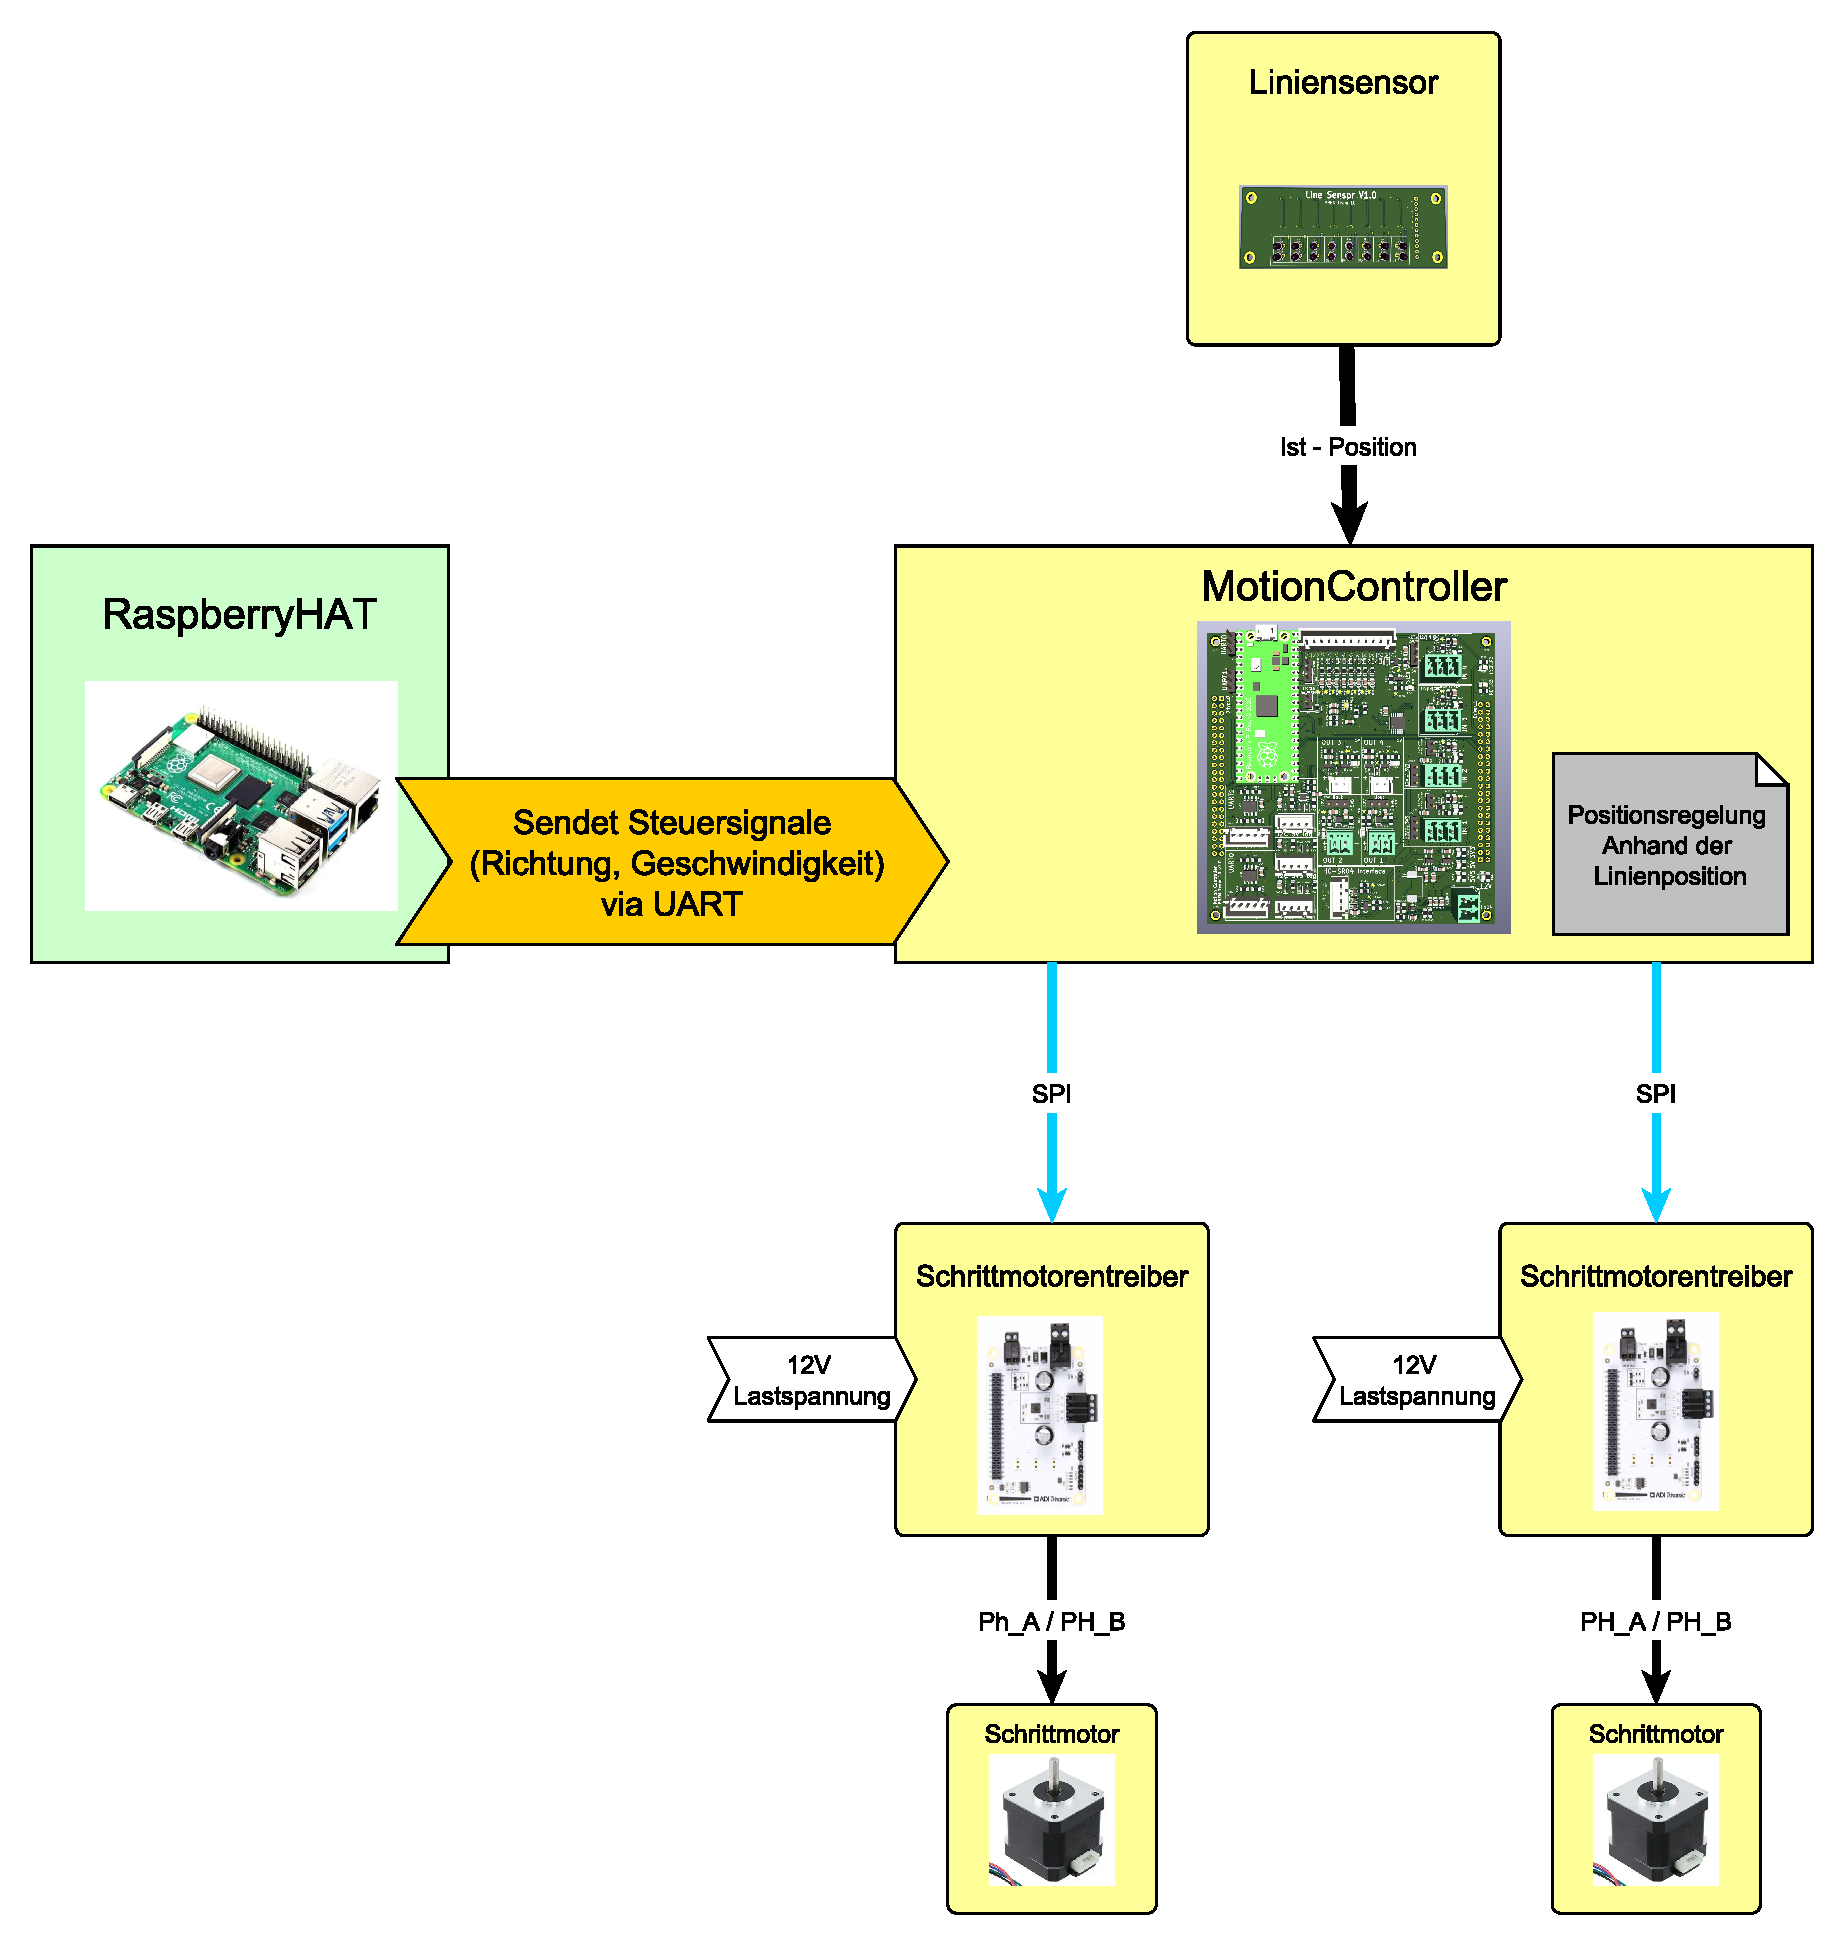
\includegraphics[width = 1\linewidth]{./fig_Antriebe/Konzept_Motoransteuerung.pdf}
    \caption{Ansteuerungstopologie Schrittmotoren}~\label{Ansteuerungstopologie_Schrittmotorentreiber}
\end{figure}

% vgl Text aus Pren1 - kann man wahrscheinlich weitestgehend übernehmen

\subsubsection*{Motoren und Motorentreiber}

Die Ansteuerung dieser Motoren erfolgt über zwei vollintegrierte
Schrittmotortreiber der Firma ADI-Trinamic. Die Ansteuerung dieser Treiber
erfolgt auf Basis der Linienposition, die über den Liniensensor ermittelt wird.
Das ist die Hauptaufgabe des Motion Controllers, wie sie im PREN1 vorgestellt
wurde.

Diese Steuerung wurde allerdings von vornherein so ausgelegt, dass sie über
mehr Ein- und Ausgänge verfügt, als benötigt werden. Durch diese
Designentscheidung kann nun auch die Aufgabe der Greifersteuerung durch den
Motion Controller übernommen werden. Für mehr Flexibilität können die Ein- und
Ausgänge auf verschiedene Spannungspegel umgeschaltet werden. Damit können
sowohl einfache 3V3 oder 5V-Sensoren als auch industrietaugliche Sensoren und
Aktoren mit 12 V Spannung betrieben werden. Auch die Arbeitsspannung der
I2C-Kommunikationsschnittstellen lässt sich konfigurieren, sodass zwischen
3,3-V- und 5-V-Logikpegeln unterschieden werden kann. Das gesamte System ist
somit sehr flexibel für etwaige Änderungen oder alternative Sensoren.

Der MotionController ist daneben allein dafür zuständig, mit Hindernissen
umzugehen. Dazu wertet er den Ultraschallsensor aus, stoppt frühzeitig und
platziert die Barriere, wie eingangs erwähnt. Alle dazu benötigten Sensoren und
Aktoren sind am Motion Controller angeschlossen.

\subsubsection{Linienfolger Regelung}

Zur Regelung der Linienposition wird ein klassischer PD-Regler eingesetzt.
Fahrten, bei denen die Regelabweichung zwingend Null sein muss, sind nicht zu
erwarten, da z.B. keine Kurven exakt abgefahren werden müssen. Ein
Integralanteil ist daher nicht erforderlich. Ausserdem zeigt der Prozess
bereits ein integrierendes Verhalten, weshalb ein I-Anteil das Regelverhalten
nachteilig beeinflussen würde.

??
%% REFERENZ AUF ABSCHNITT

Die Herleitung der benötigten Parameter ist im
Anhang~\ref{apdx:Regler_Parametrierung} detailliert beschrieben. Der Regler
wurde zunächst mit einem kleinen P-Anteil implementiert. In einem Experiment
ist die Sprungantwort des Systems aufgenommen und anschliessend mit
regelungstechnischen Methoden zu einem PT2-Modell modelliert. Dieses bildet die
Ausgangssituation für die Parameteridentifikation des implementierten Reglers.

Als Eingangsgrösse für den Regler dient die Linienposition, die direkt vom
Liniensensor geliefert wird. Die genaue Ermittlung dieser Grösse, wie genau der
Liniensensor ausgewertet wird, ist im Anhang~\ref{apdx:Liniensensor_auswertung}
beschrieben. Vereinfacht dargestellt werden die einzelnen Messzellen des
Sensors über einen ADC-Wandler ausgelesen, auf einen Vektor der Grösse $0 \dots
    1000$ normiert und anschliessend gewichtet aufsummiert. Daraus ergibt sich die
Position der Linie als ganzzahliger Wert auf einer Skala von $0 \dots 7000$,
wobei $3500$ die Mittenposition und damit die Referenzposition $x[k]$ für den
Regler darstellt.

\begin{figure}[H]
    \centering
    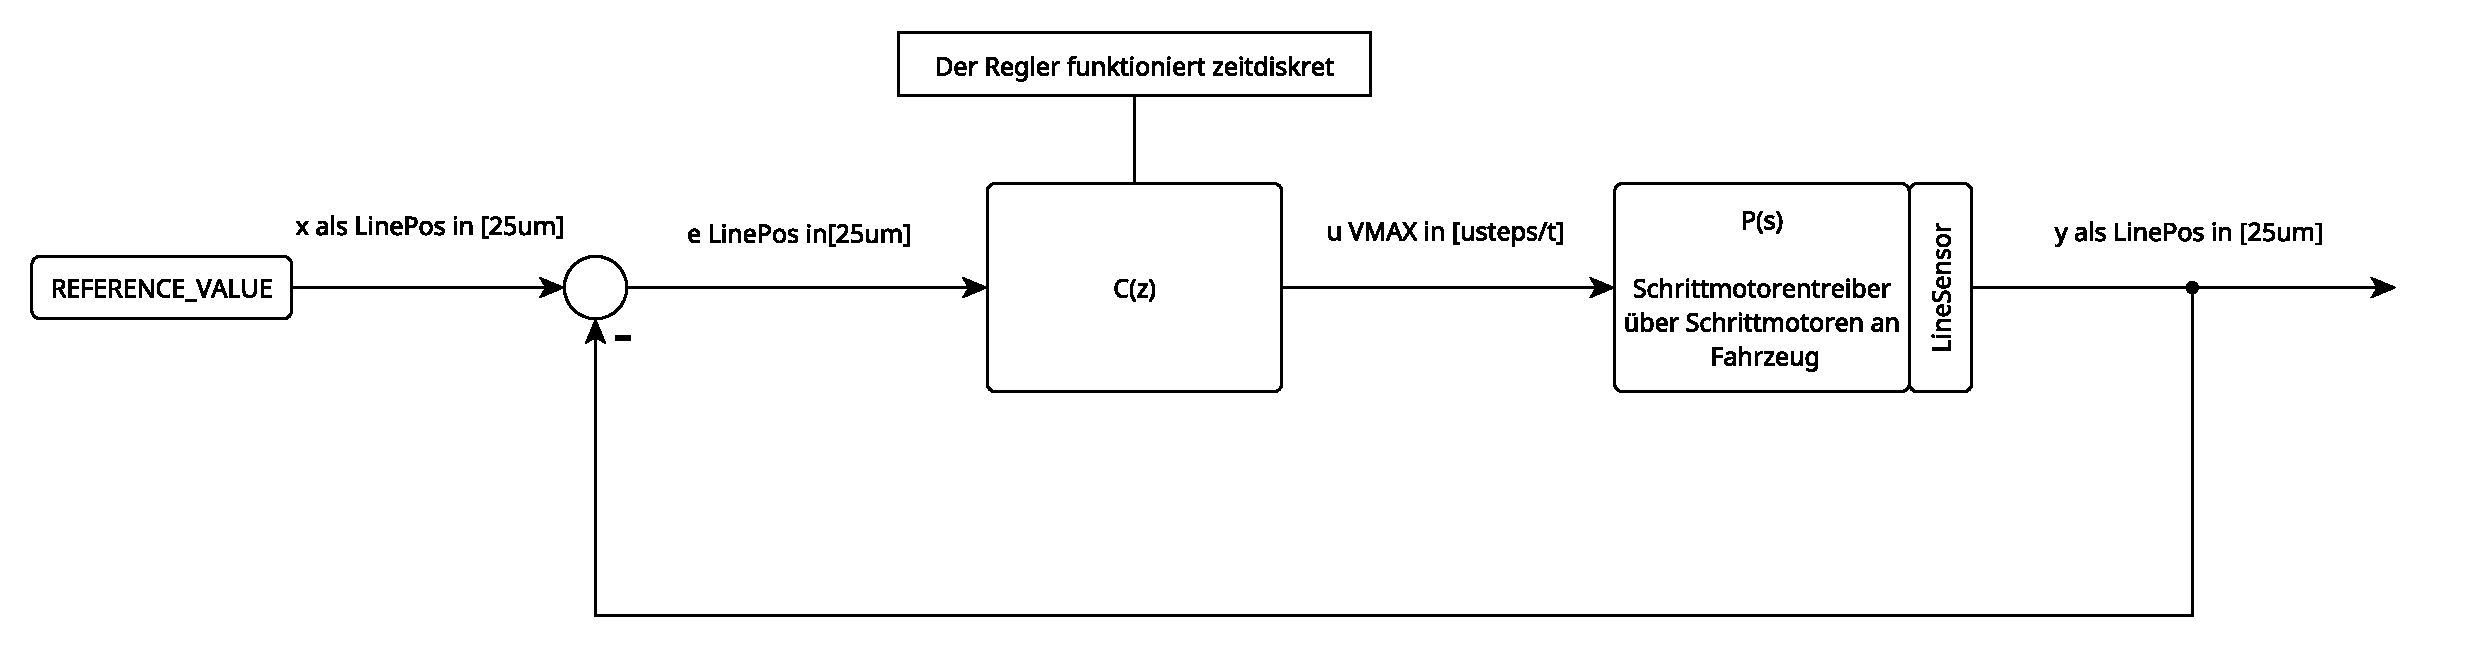
\includegraphics[width=1.0\linewidth]{../../Anhang_subfiles/Anhang_Elektronik/fig_Parametrierung_Linienfolgeregler/RegelProzess_Linienfolger.pdf}
    \caption{Reglerprozess des Linienfolgers}~\label{fig:Linienfolger_RegelProzess_ht}
\end{figure}

Der vereinfachte Regelkreis ist in
Abbildung~\ref{fig:Linienfolger_RegelProzess_ht} dargestellt. Die Grösse $x[k]$
gibt die Referenzposition an. Zusammen mit der aktuellen Linienposition $y[k]$
wird die Regelabweichung $e[k]$ berechnet. Aufgrund der Messauflösung der
Zellen haben die Werte $x[k]$, $y[k]$ und $e[k]$ alle die Einheit $25 \,\mu m$. 

Der Block $C(z)$ repräsentiert den im MotionController implementierten
zeitdiskreten Regler. Seine Ausgangsgrösse $u[k]$ hat die Einheit $\frac{\mu
        \text{steps}}{t}$

und bestimmt die Motordrehzahl, die an den Prozess $P(s)$ weitergegeben wird.
Die Ausgangsgrösse des Prozesses $P(s)$ wird dann vom Linearsensor erfasst und
durch $y[k]$ dargestellt.

Bei Geradeausfahrt wird jeder Motor mit der vorkonfigurierten maximalen
Geschwindigkeit angesteuert. Die Regelgrösse $u[k]$ wird zu einem Motor
hinzugefügt und vom anderen subtrahiert. Dadurch führt eine Regelabweichung zu
einer Drehung des Fahrzeugs um den Achsmittelpunkt.

In der Firmware des MotionControllers wurde der berechnete PD-Regler mittels
Tustin-Approximation in den zeitdiskreten Bereich übertragen. Die
Implementierung als Differenzengleichung lautet:

\[
    u[k] = \beta \cdot e[k] - \beta \cdot e[k - 1] + \alpha \cdot u[k - 1]
\]

\end{document}
